% vim: set foldmethod=marker:
%! TEX root = preprint.tex

\section{Theory}

\subsection{Representation}

Hartree--Fock wave function:
\begin{equation}
\psi_\mathrm{HF}(\mathbf r)=\det[\varphi_\mu(\mathbf r_i^\uparrow)]\det[\varphi_\mu(\mathbf r_i^\downarrow)]
\end{equation}

Backflow--Slater--Jastrow wave function:
\begin{equation}
\psi_{\boldsymbol\theta}(\mathbf r)=
\det[\varphi_\mu(\mathbf r_i^\uparrow)
  f_{\boldsymbol\theta,i\mu}(\mathbf r)]
\det[\varphi_\mu(\mathbf r_i^\downarrow)
  f_{\boldsymbol\theta,i\mu}(\mathbf r)]
\mathrm e^{\gamma(\mathbf r)+J_{\boldsymbol\theta}(\mathbf r)}
\end{equation}
where the Jastrow factor (backflow) is invariant (equivariant) with respect to same-spin electron exchange:
\begin{equation}
\begin{aligned}
J(\ldots,\mathbf r_i^\uparrow,\ldots,\mathbf r_j^\uparrow,\ldots)
&=J(\ldots,\mathbf r_j^\uparrow,\ldots,\mathbf r_i^\uparrow,\ldots) \\
\mathbf f_i(\ldots,\mathbf r_i^\uparrow,
  \ldots,\mathbf r_j^\uparrow,\ldots)
&=\mathbf f_j(\ldots,\mathbf r_j^\uparrow,
  \ldots,\mathbf r_i^\uparrow,\ldots)
\end{aligned}
\end{equation}
To preserve the cusp conditions built in $\phi_\mu$ and $\gamma$, the Jastrow factor and backflow must be cuspless,
\begin{equation}
\nabla_{\mathbf r_i}\{J,\mathbf f_j\}(\mathbf r)
  \big\rvert_{\mathbf r_i=\{\mathbf r_k,\mathbf R_a\}}=0
\end{equation}

Schnet for modeling $E(\{(t_a,\mathbf R_a)\})$:
\begin{equation}
\begin{aligned}
\mathbf x_a^{(0)}&:=\mathbf X_{\boldsymbol\theta,t_a} \\
\mathbf z_a^{(n)}&:=\sum\nolimits_{b\neq a}\operatorname{diag}
  \big[\mathbf w_{\boldsymbol\theta}^{(n)}
  \big(\mathbf e(\lvert\mathbf R_a-\mathbf R_b\rvert)\big)
  \big]\mathbf h^{(n)}_{\boldsymbol\theta}
  \big(\mathbf x_b^{(n)}\big) \\
\mathbf x_a^{(n+1)}&:=\mathbf x_a^{(n)}
  +\mathbf g_{\boldsymbol\theta}^{(n)}
  \big(\mathbf z_a^{(n)}\big) \\
E&:=\sum\nolimits_a\varepsilon_{\boldsymbol\theta}
  \big(\mathbf x_a^{(N)}\big)
\end{aligned}
\end{equation}

Schnet for electrons:
\begin{equation}
\begin{aligned}
\mathbf x_i^{(0)}&:=\mathbf X_{\boldsymbol\theta,s_i} \\
\mathbf z_i^{(n,\mathrm e)}&:=\sum\nolimits_{j\neq i}\operatorname{diag}
  \big[\mathbf w^{(n)}_{\boldsymbol\theta}
  \big(\mathbf e(\lvert\mathbf r_i-\mathbf r_j\rvert)\big)
  \big]\mathbf h_{\boldsymbol\theta}^{(n)}\big(\mathbf x_j^{(n)}\big) \\ 
\mathbf z_i^{(n,\mathrm n)}&:=\sum\nolimits_a\operatorname{diag}
  \big[\mathbf w_{\boldsymbol\theta}^{(n)}
  \big(\mathbf e(\lvert\mathbf r_i-\mathbf R_a\rvert)\big)
  \big]\mathbf Y_{\boldsymbol\theta,a} \\
\mathbf x_i^{(n+1)}&:=\mathbf x_i^{(n)}
  +\mathbf g^{(n)}_{\boldsymbol\theta}
  \big(\mathbf z_i^{(n,\mathrm e)}+\mathbf z_i^{(n,\mathrm n)}\big) \\
J&:=\eta_{\boldsymbol\theta}
  \big(\textstyle\sum_i\mathbf x_i^{(N)}\big) \\
\mathbf f_i&:=\boldsymbol\kappa_{\boldsymbol\theta}\big(\mathbf x_i^{(N)}\big)
\end{aligned}
\end{equation}

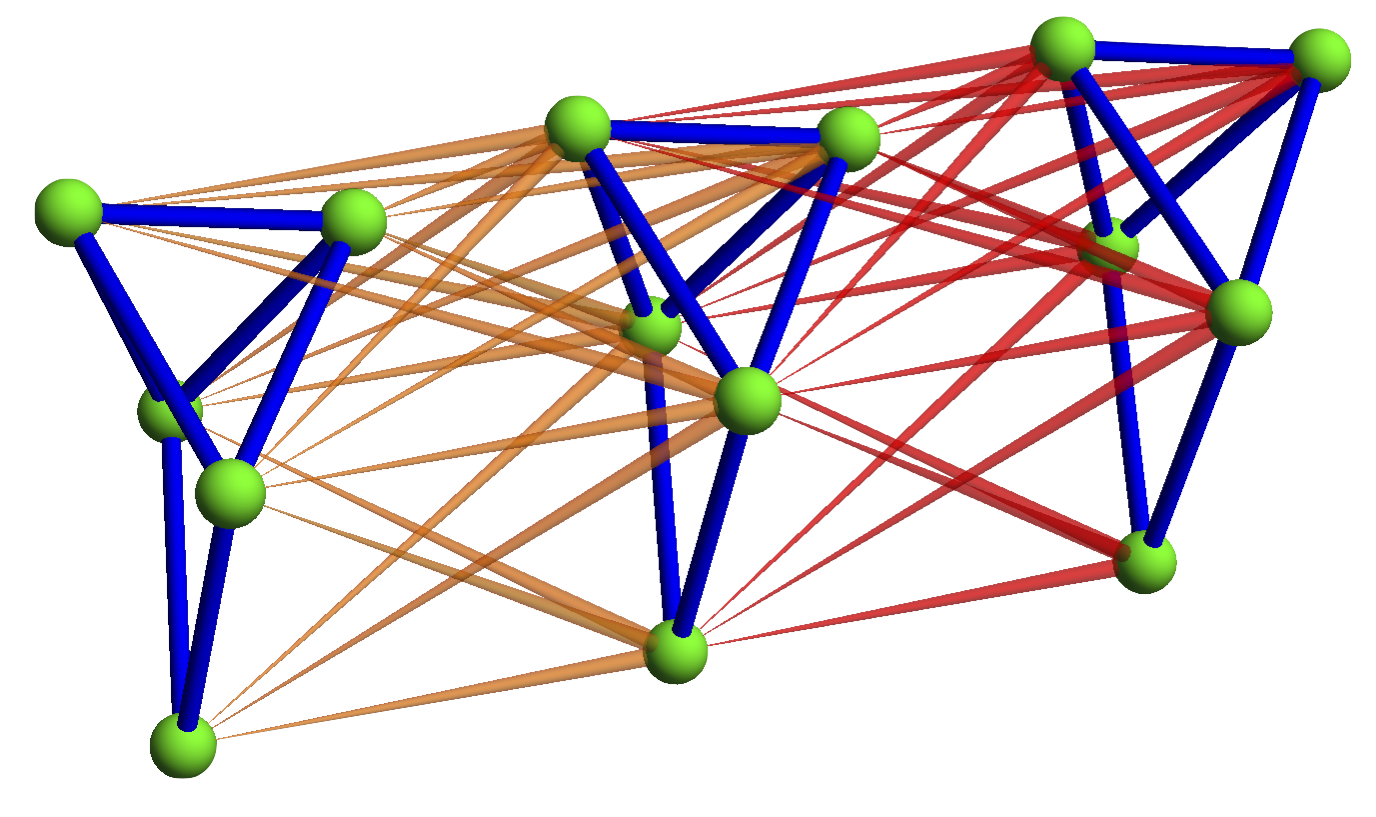
\includegraphics[width=\linewidth]{figs/gcnn.png}

Schnet for electrons version 2:
\begin{equation}
\begin{aligned}
\mathbf x_i^{(0)}&:=\mathbf X_{\boldsymbol\theta} \\
\mathbf z_i^{(n,\pm)}&:=\sum\nolimits_{j\neq i}^\pm\operatorname{diag}
  \big[\mathbf w^{(n,\pm)}_{\boldsymbol\theta}
  \big(\mathbf e(\lvert\mathbf r_i-\mathbf r_j\rvert)\big)
  \big]\mathbf h_{\boldsymbol\theta}^{(n)}\big(\mathbf x_j^{(n)}\big) \\ 
\mathbf z_i^{(n,\mathrm n)}&:=\sum\nolimits_a\operatorname{diag}
  \big[\mathbf w_{\boldsymbol\theta}^{(n,\mathrm n)}
  \big(\mathbf e(\lvert\mathbf r_i-\mathbf R_a\rvert)\big)
  \big]\mathbf Y_{\boldsymbol\theta,a} \\
\mathbf x_i^{(n+1)}&:=\mathbf x_i^{(n)}
  +\sum\nolimits_\pm\mathbf g^{(n,\pm)}_{\boldsymbol\theta}
  \big(\mathbf z_i^{(n,\pm)}\big)
  +\mathbf g^{(n,\mathrm n)}_{\boldsymbol\theta}
  \big(\mathbf z_i^{(n,\mathrm n)}\big)
\end{aligned}
\end{equation}

\subsection{Sampling}

\subsection{Training}

\section{Results}
